%% This is file `elsarticle-template-3-num.tex',
%%
%% Copyright 2009 Elsevier Ltd
%%
%% This file is part of the 'Elsarticle Bundle'.
%% ---------------------------------------------
%%
%% It may be distributed under the conditions of the LaTeX Project Public
%% License, either version 1.2 of this license or (at your option) any
%% later version.  The latest version of this license is in
%%    http://www.latex-project.org/lppl.txt
%% and version 1.2 or later is part of all distributions of LaTeX
%% version 1999/12/01 or later.
%%
%% given in the file `manifest.txt'.
%%
%% Template article for Elsevier's document class `elsarticle'
%% with numbered style bibliographic references
%%
%% $Id: elsarticle-template-3-num.tex 165 2009-10-08 07:58:10Z rishi $
%% $URL: http://lenova.river-valley.com/svn/elsbst/trunk/elsarticle-template-3-num.tex $
%%
%\documentclass[preprint,12pt]{elsarticle}

%% Use the option review to obtain double line spacing
%% \documentclass[preprint,review,12pt]{elsarticle}

%% Use the options 1p,twocolumn; 3p; 3p,twocolumn; 5p; or 5p,twocolumn
%% for a journal layout:
%% \documentclass[final,1p,times]{elsarticle}
%% \documentclass[final,1p,times,twocolumn]{elsarticle}
%% \documentclass[final,3p,times]{elsarticle}
%% \documentclass[final,3p,times,twocolumn]{elsarticle}
\documentclass[final,5p,times]{elsarticle}
%% \documentclass[final,5p,times,twocolumn]{elsarticle}

%% if you use PostScript figures in your article
%% use the graphics package for simple commands
%% \usepackage{graphics}
%% or use the graphicx package for more complicated commands
 \usepackage{graphicx}
%% or use the epsfig package if you prefer to use the old commands
%% \usepackage{epsfig}

%% The amssymb package provides various useful mathematical symbols
\usepackage{amssymb}
\usepackage{amsmath}
%% The amsthm package provides extended theorem environments
%% \usepackage{amsthm}

%% The numcompress package shorten the last page in references.
%% `nodots' option removes dots from firstnames in references.
\usepackage[nodots]{numcompress}

%% The lineno packages adds line numbers. Start line numbering with
%% \begin{linenumbers}, end it with \end{linenumbers}. Or switch it on
%% for the whole article with \linenumbers after \end{frontmatter}.
\usepackage{lineno}

%% Avoids linenumbers to collide with text for 5p format:
\setlength\linenumbersep{3pt}

%% natbib.sty is loaded by default. However, natbib options can be
%% provided with \biboptions{...} command. Following options are
%% valid:

%%   round  -  round parentheses are used (default)
%%   square -  square brackets are used   [option]
%%   curly  -  curly braces are used      {option}
%%   angle  -  angle brackets are used    <option>
%%   semicolon  -  multiple citations separated by semi-colon
%%   colon  - same as semicolon, an earlier confusion
%%   comma  -  separated by comma
%%   numbers-  selects numerical citations
%%   super  -  numerical citations as superscripts
%%   sort   -  sorts multiple citations according to order in ref. list
%%   sort&compress   -  like sort, but also compresses numerical citations
%%   compress - compresses without sorting
%%
%% \biboptions{comma,round}

% \biboptions{}


\journal{Computers \& Graphics}

\begin{document}

\begin{frontmatter}

%% Title, authors and addresses

%% use the tnoteref command within \title for footnotes;
%% use the tnotetext command for the associated footnote;
%% use the fnref command within \author or \address for footnotes;
%% use the fntext command for the associated footnote;
%% use the corref command within \author for corresponding author footnotes;
%% use the cortext command for the associated footnote;
%% use the ead command for the email address,
%% and the form \ead[url] for the home page:
%%
%% \ title{Title\tnoteref{label1}}
%% \tnotetext[label1]{}
%% \ead{email address}
%% \ead[url]{home page}
%% \fntext[label2]{}
%% \cortext[cor1]{}
%% \address{Address\fnref{label3}}
%% \fntext[label3]{}

\title{Procedural Bread Making}

%% use optional labels to link authors explicitly to addresses:
%% \author[label1,label2]{<author name>}
%% \address[label1]{<address>}
%% \address[label2]{<address>}

\author{}

\address{}

\begin{abstract}
%% Text of abstract

\end{abstract}

\begin{keyword}
%% keywords here, in the form: keyword \sep keyword

%% MSC codes here, in the form: \MSC code \sep code
%% or \MSC[2008] code \sep code (2000 is the default)

\end{keyword}

\end{frontmatter}

%%
%% Start line numbering here if you want
%%
\linenumbers

%% main text
\section{Introduction}


\section{Previous Work}
Accurate geometry models are main requirements in material modeling and rendering \cite{Dorsey2007}. 

Procedural geometric modeling avoids the need for artistical intervention in large domains: cities \cite{Parish2001}, planets \cite{Ebert2002}, buildings \cite{Muller2006}, and plants \cite{Prusinkiewicz1990}. These methods use grammars to define mathematical descriptions representing spatial relationships between primitives - cubes, cilynders, lines-. The final structure arises using recursion over grammar elements.

Bread geometric modeling is a multidisciplinary research topic. On the one hand, the computer graphics area shows some initial work on bread crumb modeling and rendering \cite{Tong2005,Cho2007}.  Bread making involves several stages that are usually ignored or poorly studied in computer graphics modeling.

On the other hand, food engineering literature shows that the proving stage of bread making strongly determines bubble distributions in bread crumbs \cite{Babin2006}. In this step, interaction between the yeast and the dough produces {\em $CO_{2}$}. Bubble radius differs in the dough, making it a fractal-like structure: the structure repeats itself or is statistically similar at different measurement scales. Studies computed different fractal dimensions for these structures in certain bread types \cite{Gonzales2008}, suggesting a fractal bubble distribution.

Previous studies in fractals proposed a model to capture natural phenomena such as moon craters and bubble size distribution in cheeses \cite{Mandelbrot1982}. The author defines radius for circles subtracting them from a white image using the relationship $r = Q/\sqrt{p}$, where $p$ is a random natural number, $r$ is the radius of the subtracted circle and $Q$ is a parameter determining the fractal dimension of the remaining image (the black region). This fractal dimension is equal to $2-2\pi Q^{2}$.

In addition, complex mathematical models represents the behaviour and growing of several natural phenomena. In computer graphics, some work used them to model water and fluids \cite{Stam1999,Fedkiw2001}. Authors borrow differential equations from other science fields and approximate them using numerical techniques. In recent years, GPGPU technology \cite{Owens2007} made them available for use at interactive or real time rates.

In bread modeling, the rendering stage also presents several challenges since it shows complex light phenomena: self-occlusion, self-shadowing, transmittance and reflection, among others. Some studies introduced complex solutions for its rendering \cite{Tong2005}. Nevertheless, such procedures need a complex equipment and set up, limiting the result to one capture. 

For bread crumbs it is crucial to simultaneously generate an accurate geometry model and represent the material's light interaction. Literature shows only a few approaches to manage both situations using artistical considerations \cite{Cho2007}. Nevertheless, the authors did not publish enough details of the model and rendering since a private movies company developed the method. A previous work applied a mathematical model of baking to certain bread types for rendering animations \cite{Rodriguez-Arenas2011}, but they did not address the breads crumb bubbles' geometry.

Deformation is an approach to gain modeling flexibility. Literature shows methods for geometrical deformations \cite{Lipman2008,Floater2003}. These techniques uses cages with user defined control points to perform deformations. Changing the control points, it is possible to perform natural animations using only one geometry, allowing artists to participate in the process.

Here we propose to unify and clearly differentiate the key steps of bread making (proving, baking, human deformation) to produce a physically correct pipeline for procedural generation of bread crumb geometries. Using this approach, we follow the ideas of Predictive Rendering \cite{Wilkie2009}, using mathematical models to make physically correct simulations. Next section introduces the theory for the model.

\section{Mathematical background}

\subsection{Bread baking mathematical model}
Bread baking mathematical models adequately simulates heat and mass transfer in dough. The mathematical model consists of three coupled set of equations describing heat transfer, water vapour diffusion and liquid water diffusion. In our algorithm,  we use only the temperatures ($T$) as the input for the next stage. The next differential equation models heat transfer in bread dough:

\begin{equation}
\frac{\partial T}{\partial t} = \frac{1}{\rho C_{p}} \frac{\partial}{\partial x} \left ( k \frac{\partial T}{\partial x} \right ) + \frac{\lambda}{c_{p}} \frac{\partial W}{\partial t}+\frac{\lambda W}{ C_{p} \rho}\frac{\partial \rho}{\partial t},
\end{equation}


\noindent where $T$ is temperature, $x$ is the space coordinate, $C_{p}$ is the specific heat, $\rho$ is density, $k$ is thermal conductivity and $\lambda$ is the latent heat of evaporation of water. The initial conditions,

\begin{align}
\left ( \frac{\partial T}{\partial x} \right )_{x=L/2} &= 0 , t > 0, \\
T(x,0) &= T_{x}(0), 0\le x \le L/2,\\
\end{align}
and the boundary conditions define the model:
\begin{align}
-k \left ( \frac{\partial T}{\partial x} \right )_{x=0} &= h_{r}(T_{r}-T_{s}) + h_{c}(T_{air}-T_{s}) - \lambda \rho D_{w} \left (\frac{\partial W}{\partial x} \right )_{x=0},
\end{align}

\noindent where $h_{r}$ and $h_{c}$ are subterms of the heat transfer coefficient ($h = h_{r}+h_{c}$), $T_{air}$, $T_{s}$, $T_{r}$ are the temperatures in the surrounding air, at the surface of the bread and at the radiation source, respectively. The model presents similar equations for water vapour diffusion ($W$) and  liquid water diffusion ($V$). Further details of this model can be seen in \cite{Powathil2004}.

\subsection{Mean Value Coordinates}
We add user interaction within our model by letting the user move control points in the dough, emulating baker's dough deformation.

Mean Value Coordinates (MVC) is a powerful tool for animation \cite{Floater2003,Floater2005,Ju2005}.  This method uses control points to change structure positions, deforming the volume. It uses barycentric coordinates to compute the new deformed positions of every point in the original structure.

MVC uses two control point sets for warping. The first one ($cageOrig$) is a point set lying in the original image boundary.  Each texel computes its barycentric coordinates with respect to these points. When we move these points ($cageNew$), the method multiplies the barycentric coordinates with the perturbed control points for each texel:

\begin{align}
barycoords &= MVC([x,y],cageOrig),\\
(u,v) &= \sum_{i} {barycoords_{i} * cageNew_{i}}, \\
T(x,y) &= T(u,v).
\end{align}
As the reader will see in next sections, this method produces realistic-looking deformations.

\subsection{Multifractal theory}

Fractal dimensions (FD) measure key image features in narrow representations. Several FDs capture different features, {\em e.g.}, porosity, rugosity, etc.) . Studies shows fractal bread characterisations using several FDs \cite{Gonzales2008,Baravalle2012}. 

Literature shows different representations for the multifractal spectrum. The different representations provide identical information and differ only for a Legendre transformation. There are two main classes of multifractal spectra: generalised multifractal dimensions and . This transformation boost the performance in classification tasks.

Studies compute generalised multifractal dimensions  in several ways. The Sandbox multifractal method \cite{Tel1989} aims to compute the dimensions using the meaning value in a set of randomly distributed points belonging to the structure \cite{Debartolo2004}. The author defines the sandbox multifractal dimension of order q as:

 \begin{align}
D_{q\ne 1}^{sb} &= \frac{1}{q-1} \lim_{R \rightarrow 0}{
\frac{ln   { \left\langle  (M(R)/M_{0})^{q-1} \right\rangle   }}
{ln {(R/L)}       }},\\
D_{q=1}^{sb} &= \lim_{R \rightarrow 0}{
\frac{ \left\langle ln   { (M(R)/M_{0})  }  \right\rangle}
{ln {(R/L)}       }},
\end{align}

\noindent where $M_{0}$ is white pixels count in the image binarization and  $M(R)$ is the number of points belonging to the structure in a circle of radius $R$ centered at the $i$ point. When $q\ne1$, we compute the limit as the slope of the linear fit of the values $ln(R/L)$ vs. $ \left\langle ln   { (M(R)/M_{0})  }  \right\rangle$, for $R$ in $[R_{min}, R_{max}]$, where $ \left\langle   \right\rangle$ denotes mean value over sampled points. We proceed similarly when $q=1$. Computing the value for different $q \in [-Q,Q]$  we obtain the sandbox spectrum.


The Multifractal Spectrum (MFS) \cite{Xu2009} applies a pixel based discrimination using pixel neighborhood information. The discrimination produces different substructures in the image characterised by a local scaling $\alpha$ exponent. The method obtains the Box FD \cite{Peitgen2004} for each structure. This produces a vector of fractal dimensions $f(\alpha)$, meaning that different fractals coexists in the structure.

We compute the local scaling exponent $\alpha$ for every pixel in the following way: we divide the structure $E$ in disjoint substructures $E_{i}$ of size $\varepsilon$ characterised by a measure $\mu(E_{i})$, and we define the H\"older exponent, $\alpha_{i}$, for each substructure $E_{i}$, as a function of $\varepsilon$, 
 \begin{align}
\alpha_{i} &= \frac{ln(\mu(E_{i}))}{ln(\varepsilon)},\\
\alpha &= \lim_{\varepsilon\to0}{\alpha_{i}}.
\label{eqn:eqn4}
\end{align}
In our case, we define $\mu$ as the image intensity. We compute an $\alpha$ exponent for every pixel. We obtain the MFS computing the Box Dimension of the sub structures characterised by different $\alpha$ under different real ranges. For each range, the (multi) fractal dimension $f(\alpha_{i})$ of the resulting structure is:
\begin{align}
f_{\varepsilon}(\alpha_{i}) &= - \frac{ln(N_{\varepsilon}(\alpha_{i}))}{ln(\varepsilon)},\\
f(\alpha_{i}) &= \lim_{\varepsilon\to0}{f_{\varepsilon}(\alpha_{i})}.
\end{align}
\noindent where $N_{\varepsilon}(\alpha_{i})$is the number of points in a circle of radius $\varepsilon$ centered at the pixel with exponent $\alpha_{i}$. In practice we compute $f(\alpha)$ as the (negative) slope of the linear fit between the values of $\varepsilon$ and $N_{\varepsilon}(\alpha_{i})$.

The MFS and the sanbox spectrum are related via a Legendre Transform. We can compute the MFS using the Legendre transform of the sandbox spectrum or we can compute it directly from the underlying structure. The latter gives better classification performance. In our experiments, we use the latter approach to compute the MFS for reañ and rendered bread images, and we apply the sandbox approach to characterise real and synthetic bread binarisations.

Next sections introduces our algorithm's pipeline.




\section{Bread making algorithm}

\begin{figure}
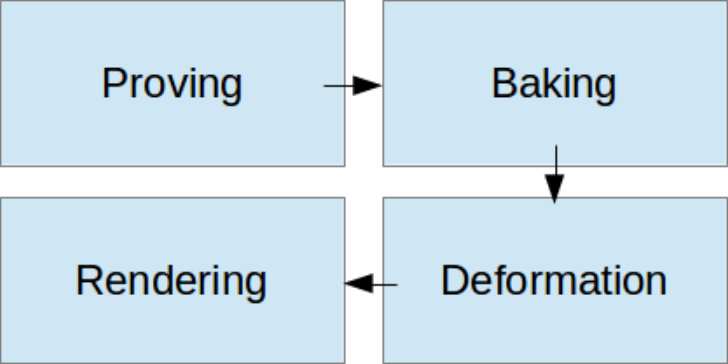
\includegraphics[scale=0.45]{pipeline.png}
\caption{Pipeline for synthetic bread making.}
\label{FigPipeline}
\end{figure}

Fig~\ref{FigPipeline} outlines our model's  pipeline. It consists of $4$ sequential stages emulating bread making. The first step introduces an algorithm for bread proving simulation. Then we apply the bread baking mathematical model \cite{Powathil2004} to slightly deform the bubbles. The third step employs Mean Value Coordinates (MVC) \cite{Floater2003} for an user defined warping of the resulting structure. Finally we apply direct volume rendering \cite{Kruger2003} getting realistic images of the process.

The proving step is defined in a $3D$ cube. We apply the baking and deformation steps to resulting $2D$ volume slices, since the baking model is cilyndrical (the properties are constant in the $Z$ coordinate).


The next subsection shows the first stage of this pipeline.

\subsection{Proving simulation}
\label{breadprov}
Bubble patterns in bread result from complex processes: chemical reactions and physical deformations in bread dough. Bread making involves two sequential sub-processes: {\em proving} \cite{Babin2006} and {\em baking} \cite{Mondal2008}. Proving accounts for free bubble growth produced by living yeast in dough. Then, human intervention deforms dough shapes in several ways. The baking process gives the final bubbles' shape.

Phenomenological studies of bubble distribution employed X-ray tomography devices and image feature extraction \cite{Babin2006, VanDyck2014,  Gonzales2008}. Despite its accuracy, this method fixs the structure with the capture.

To obtain structure variability, we generate bubbles distributions with a fractal-based model \cite{Mandelbrot1982} and we validate them using the sandbox multifractal spectrum.

We introduce a model in space using these ideas. We start with an sphere with initial radius of $v$ voxel and then we increment it. The number of spheres we extract in each step is proportional to the radius in the following way:

\begin{equation}
N_{spheres} = \frac{k}{r^{d}} ,
\end{equation}

\noindent where $k$ and $d$ are real-valued parameters, and  $r$ is the sphere radius. Fig.~\ref{FigProving} shows a $2D$ example of our model.  The parameter $d$ controls the decreasing relationship of increasing radius. $k$ controls the amount of spheres we introduce in each step.

Images show high resemblance in size distribution with real bread proving binarisations (see \cite{Babin2006}). We will compute similar parameter values to real bread crumbs in the validation section.


Next subsection explains the application of the bread baking process to this structure.


\begin{figure}
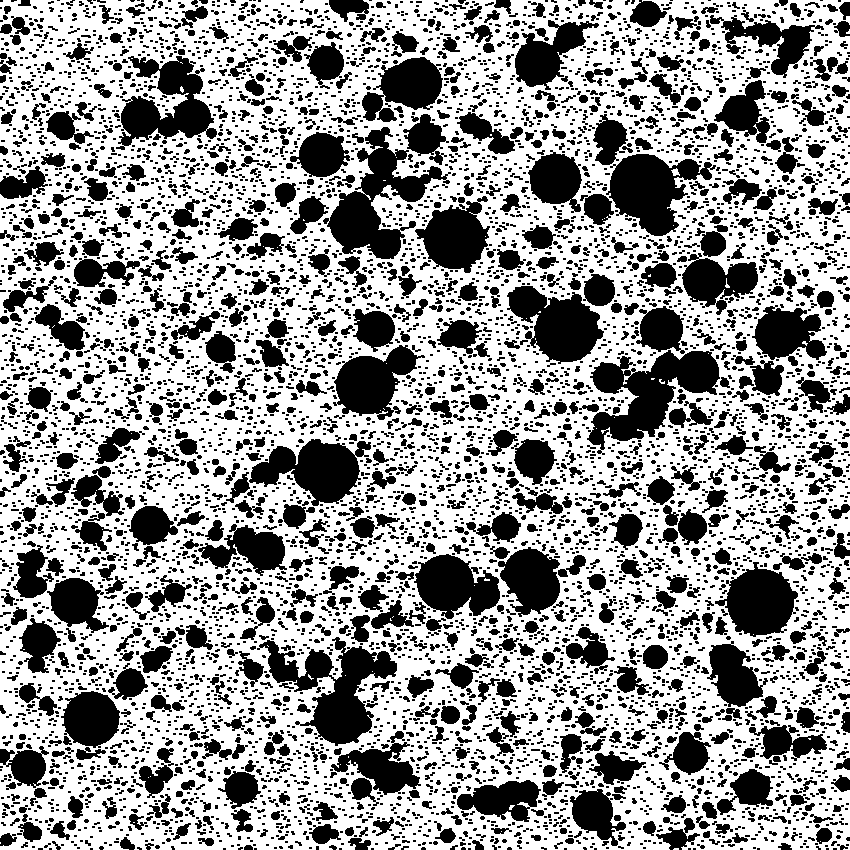
\includegraphics[scale=0.28]{bubbles.png}
\caption{Fractal bread proving simulation.}
\label{FigProving}
\end{figure}


\subsection{Baking simulation}
In our case, a simple one dimensional representation suffices \cite{Powathil2004,Purlis2010}  since the baking effect in bubbles' shape is the lowest in the bread making pipeline. 

We use the numerical implementation in \cite{Powathil2004} that is based on the finite differences scheme. 

The baking simulation sets an oven at $210°C$ and discretises time in intervals of length $\Delta t$.  We obtain an array of $N$ temperature values. Each value represents a dough position after $M$ baking time steps. For more stable results, we set $N=32$.

We translate this vector into $2D$ coordinates using the following relationship:
\begin{equation}
R = \sqrt{x^{2}+y^{2}},
\end{equation}


\noindent where $R$ is the vector index, and $x$ and $y$ are $2D$ coordinates in the resulting image, {\em i.e.}, we set the image pixel $I(x,y)$ with $v[R]$. Fig.~\ref{FigBakingVectorField} shows the result of this process.

We compute a vector field $[g_{x},g_{y}]$ from the image gradient \cite{Gonzalez2006}, and we use it to warp the volume texture in the following way:

\begin{align}
u = x+g_{x}[x,y],\\
v = y+g_{y}[x,y],
\end{align}
\noindent where $(u,v)$ are the coordinates in the warped image and ($x,y$) are the original image coordinates. Fig.~\ref{FigBakingVectorField} also shows the computed gradient. Since our temperature result is constant modulus $32$, we interpolate the values to get coarser grids.


\begin{figure}
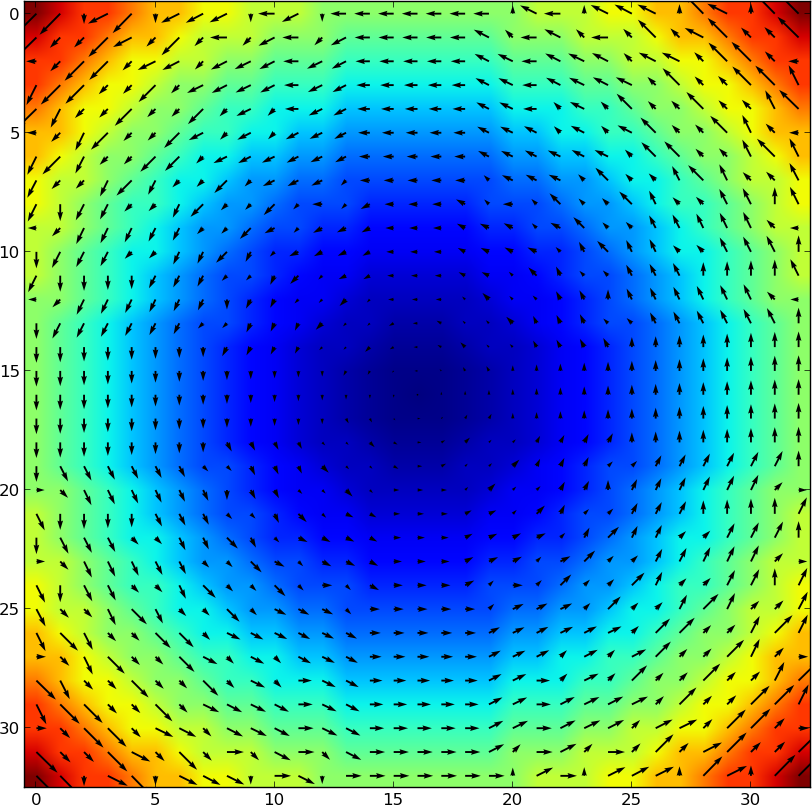
\includegraphics[scale=0.58]{vfield.png}
\caption{Temperatures from the bread baking mathematical model and superimposed gradient vector field .}
\label{FigBakingVectorField}
\end{figure}

Arrow length indicates vector modulus. The image shows that the field's influence is higher near the crust, mostly deforming outer bubbles. This behaviour is consistent with real bread crumbs: baking influences the outer bubbles' shape, elongating them parallel to the crust \cite{Scanlon2001}, in other words, following its isotherms.

Since we defined a cilyndrical bread model and only a few slices suffices for bread visualization, we use a $2D$ model and we warp each volume texture slice independently of each other, obtaining the final {\em baked} volume. Fig.~\ref{FigBaking} shows a slice result example of this process. Further work may use a $3D$ baking model.  

\begin{figure}
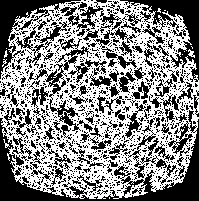
\includegraphics[scale=0.95]{baking.png}
\caption{Volume slice after baking.}
\label{FigBaking}
\end{figure}

Next subsection shows the final texture warping, emulating human intervention in dough.


\subsection{Volume Warping}
In this stage an artist can define control points in an image, changing its external shape to produce natural bread crust silhouettes. 


Based on our cilyndrical assumption, we apply the warping separatedly for each slice. Future work can define a $3D$ cages model for our process.


Fig.~\ref{FigMVC} shows a warping example using MVC. In that case, $11$ control points were enough to approximate the real crust shape. Fig.~\ref{FigMVCpoints} shows the control points and the deformed cage. In the example we put more points in the region of interest (right) to produce a more controlled deformation than in the left region.

\begin{figure}[!ht]
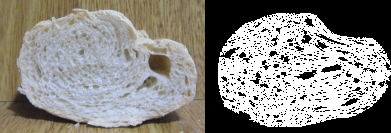
\includegraphics[scale=0.65]{warping.png}
\caption{Image warped using mean value voordinates. The image also shows a real bread image to the left. }
\label{FigMVC}
\end{figure}


\begin{figure}[!ht]
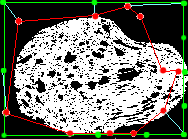
\includegraphics[scale=1.35]{warppoints.png}
\caption{Image warped, original control points (green) and moved control points (red). Other lines indicate point displacements. }
\label{FigMVCpoints}
\end{figure}


This method also warps the bubbles' shape. The deformed bubbles have a natural appearance in concordance with real bread bubbles. 


We apply this step after baking to mantain simplicity in the baking step: if we invert the order, the baking model should be nonlinear due to the external shape produced. In real bread making, baking takes place after proving. Our pipeline inverts baking and human deformation. The results we obtained suggests that the inversion produce adequate images for our purposes.

Next section shows rendering results and the fractal model validation.

\section{Results}
In this section we present the results of our procedural bread making pipeline and we validate the model using multifractal feature extraction.

\subsection{Rendering}
This step's purpose is the model visualization and image validation.

Direct volume rendering (DVR) \cite{Levoy1988, Max1995,Kruger2003} approximates the light transport equation by throwing rays into a volume from a virtual camera, accumulating density information. The process forms an image from a camera positioned in space.

We prefer DVR over other state-of-the-art methods such as Ray Tracing \cite{Whitted1980,Singh2010}, Path Tracing \cite{Lafortune1993} and Photon Mapping \cite{Jensen1996}, since they are computationally expensive and they require a detailed object mesh.

Fig.~\ref{FigRenders} shows DVR-rendered images  of the bread making algorithm we presented in this work. Images show a realistic bread crumb appearance, suitable for photo-realistic rendering and serious games \cite{Susi2007}.

\begin{figure}[!ht]
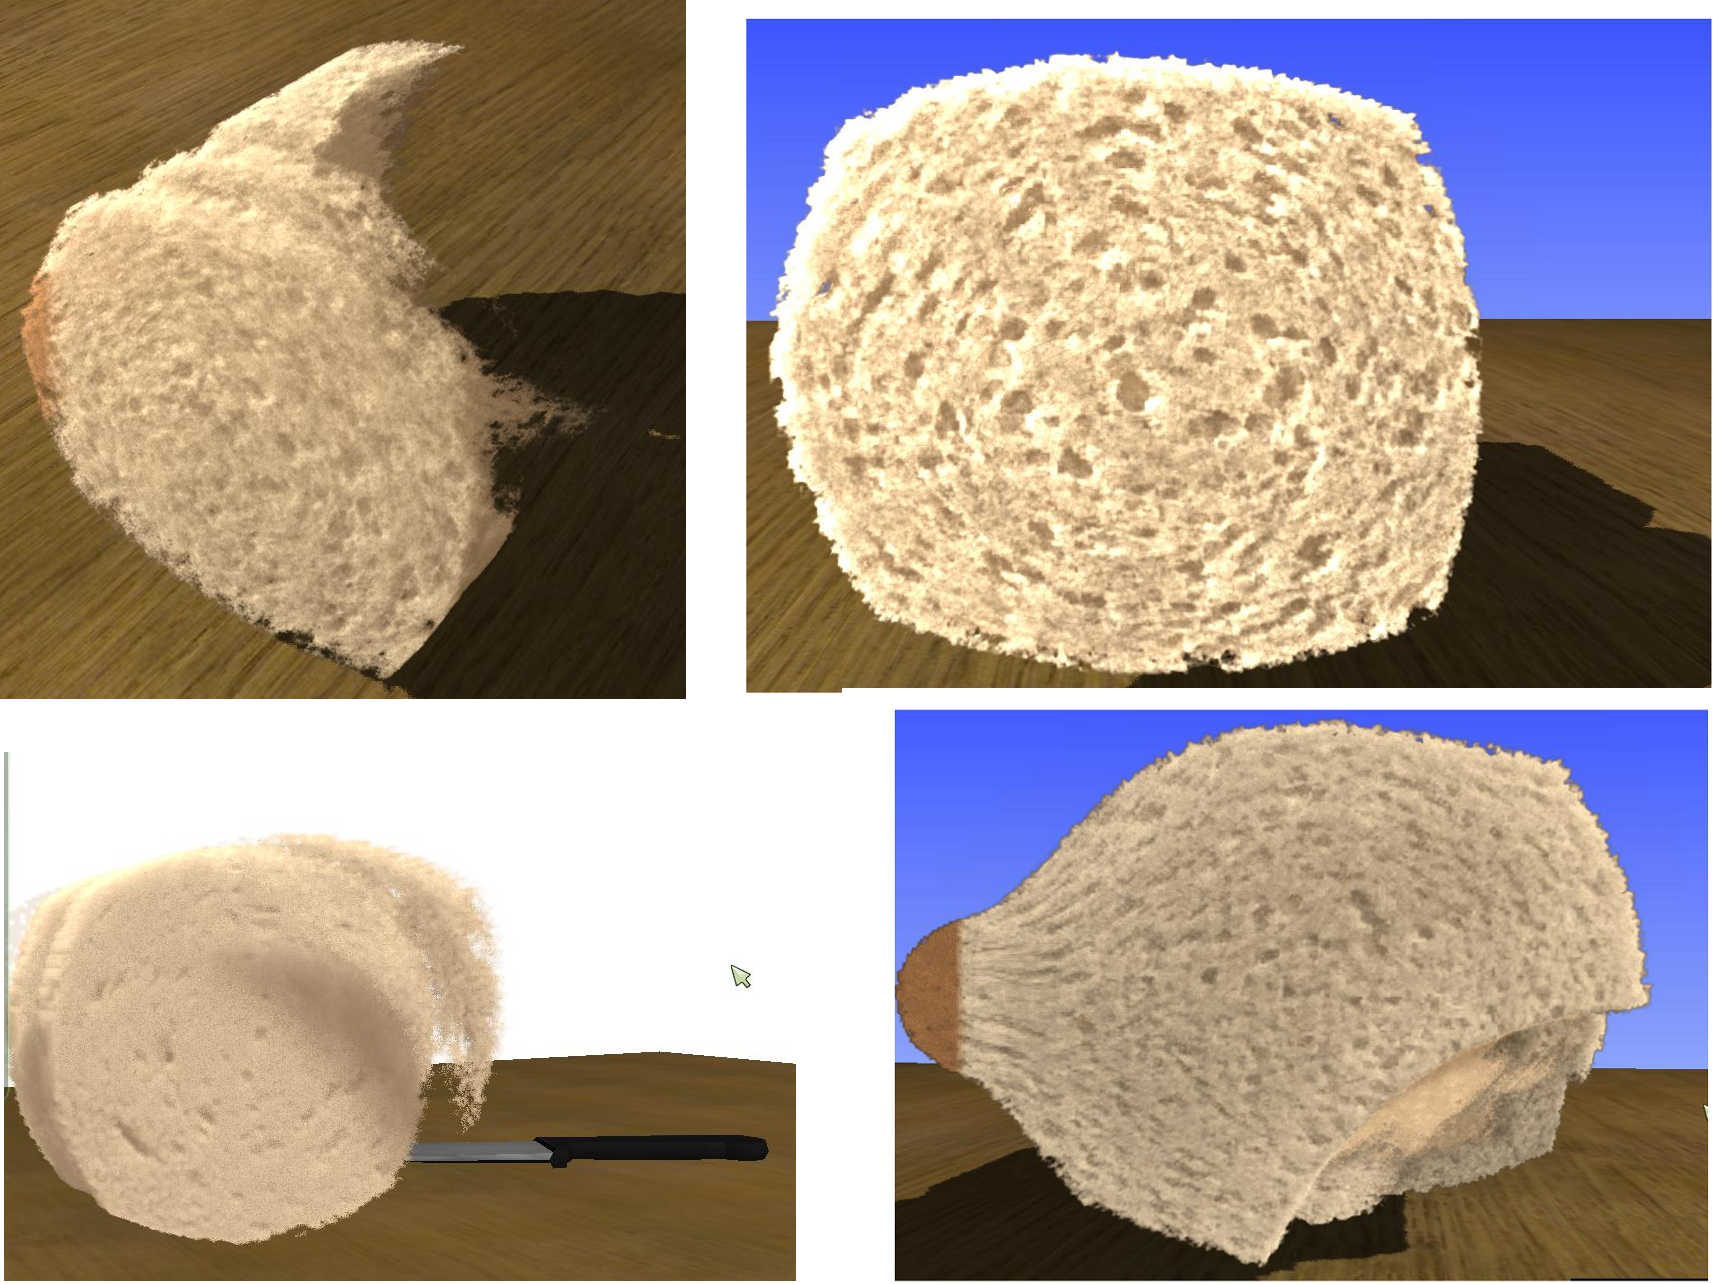
\includegraphics[scale=0.15]{render2.png}
\caption{DVR synthetic bread crumb renders}
\label{FigRenders}
\end{figure}

The authors have used physically correct mathematical models constructing a multi-step pipeline in synthetic bread crumb modelling and visualization. 

Next section validates this model using fractal methods.

\subsection{Model Validation}

First we apply the sandbox multifractal method to study the geometry we obtained after the deformation step. The method is best suited for geometrical structure characterisation.

We apply the sandbox method to $10$ binarised real bread crumb images that we captured with a digital camera and $10$ syhthetic images produced using our pipeline, obtaining $20$ feature vectors. Then we separate each class and we compute boxplots for the two classes. We manually segmented real bread crumbs to prevent automatic segmentation errors as in \cite{Bosch2011}. The model has $5$ parameters:


\begin{align}
N_{spheres} &= \frac{k}{r^{d}},\\ r &= v_{min}+step*j,\\ r &\le v_{max} 
\end{align}
$k,d,v_{min},v_{max}$ and $step$, which controls bubble's generation in the proving step. We implemented an automated search in parameter space and we found that the following parameters produce the lowest error:

\begin{align*}
k &= 0.04\times N\times N\times N ,\\
d &=2.8,\\
v_{min} &=2,\\
v_{max} &=40.\\
step &=1.
\end{align*}

The accumulated error in medians is $0.98$. We compute this error as $\displaystyle \sum abs(means_{real}-means_{synthetic})$. Fig.~\ref{FigBoxPlots} shows boxplots of real and synthetic breads. When $q < 0$ dimensions have a higher dispersion, since the method approximates these dimensions less accurately. The figure shows strong similarities between real and synthetic spectrums.  Fig.~\ref{bincomparison} shows an example of real and synthetic binarisations for these parameters.

Automated searchs in parameter space may be useful to automatically match other bread types and materials.

To test the rendering algorithm, we employ the Multifractal Spectrum (MFS) \cite{Xu2009}. This method can distinguish bread crumb from non-bread crumb images with high accuracy  \cite{Baravalle2012}.

SOM maps \cite{Kohonen2001} reduces the N-dimensional feature space into a two dimensional representation while mantaining neighborhood information. These maps allow to see feature vectors distributions in space in a human-useful representation.

Fig.~\ref{FigSOM} shows the SOM map for the MFS image representation. We compute the MFS in the $80$ images obtaining a feature vector for each of them. We use these vectors to populate the map. The map we obtained presents evidence for bread and non-bread separability since each class' vectors is separable.

\begin{figure}[h!]
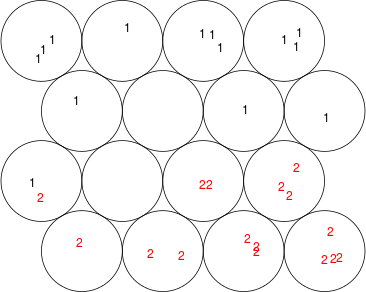
\includegraphics[scale=0.65]{som.png}
\caption{Self Organising Maps showing bread and non-bread separability. 1: Bread, 2: Non-bread }
\label{FigSOM}
\end{figure}

For the sake of completion. we also set a simple experiment to validate synthetic images produced using our rendering method: $20$ real bread crumb images captured with a digital camera and $20$ non-bread images from a public dataset \cite{FeiFei2004} train a Random Forests (RF) \cite{Breiman2001} and Support Vector Machines (SVM) \cite{Vapnik1995} defining $2$ balanced classes. Twenty synthetic images obtained using our method and $20$ non-bread images from the same public dataset defines the test set. We manually segmented real and synthetic bread crumbs to prevent automatic segmentation errors as in \cite{Bosch2011}.


Table~\ref{Table1} shows the classifiers' performance (the percentage of correct classifications in the test set). Table~\ref{Table2} shows the SVM classifier confusion matrix: each row represents the correct class, and each column the classifier result; a diagonal matrix means the classifier performed optimally.

\begin{table}[htb]
\centering
\begin{tabular}{c|c}
\hline
 Method & Accuracy  \\
\hline
 RF & 77.5 \% \\
SVM  & 87.5 \% \\
\hline
\end{tabular}
\caption{Classification performance }
\label{Table1}
\end{table}

\begin{table}[htb]
\centering
\begin{tabular}{c|c|c}
\hline
 Class & bread & non-bread  \\
 \hline
bread & 18 & 2  \\
 non-bread & 3 & 17  \\
 \hline
\end{tabular}
\caption{Confusion matrix for the SVM classifier}
\label{Table2}
\end{table}

\begin{table}[htb]
\centering
\begin{tabular}{c|c|c}
\hline
 Class & bread & non-bread  \\
 \hline
bread & 13 & 7  \\
 non-bread & 2 & 18  \\
 \hline
\end{tabular}
\caption{Confusion matrix for the random forests classifier}
\label{Table3}
\end{table}

An automatic robust classifier classifies most synthetic images as real bread images (the classifiers detected $2$ and $7$ as synthetic).

Based on these tests, we believe that our procedure adequately models bread crumbs structures. The Sandbox multifractal method and the MFS detect compatible fractal patterns in our synthetic images and in real bread crumbs, suggesting the correctness of the bubble size distributions' model.


\section{Discussion}
We introduce a pipeline to model realistic bread crumb geometry based on a fractal generation procedure. The $4$ different stages flexibilised the model, allowing to tune and test each of them separatedly.

We designed the proving step inspirated in Mandelbrot's model for moon's craters and cheeses bubbles. These patterns can be used in several other materials involving bubbles such as foams and sponges. The visual texture can be enhanced using self-avoiding bubbles, but this requires higher computing time. We defined different parameters related to the bubble radius, amount and its relationship.

The original baking model is $1D$. We used the temperatures information  and we translated them to $2D$ coordinates using euclidean distance to the $2D$ origin. We defined a cilyndrical $3D$ model setting constant properties for the $Z$ coordinate. 

The baking-deformation inversion we introduced eliminates the neccesity of $3D$ baking models, reducing the model complexity and the computing resources needed. The $2D$ simplification of the deformation step agreed with our cilyndrical model and showed acceptable results in bubble global and local deformations. This  deformation limitation can be extended to $3D$ in a future work.

We performed two tests to validate the model after two pipeline steps: deformation and rendering. The first test used the Sanbox method, best suited for geometrical multifractals, and obtained synthetic spectra with low error rates when compared to real spectra.  These results indicates that the bubble's proving model concordates with real bread crumbs bubbles distribution (amounts and sizes of bubbles). 
We found higher dispersion in the negative dimensions ($q \ge 0$), since the method better approximates the positive generalised multifractal dimensions. 

The second test employed the MFS to validate the suitability of the pipeline in a typical rendering system. We also obtained low error rates in classification performance using two different classifiers. The SOM maps of the feature space shows the separability of bread and nonbread images. This indicates our rendering system is producing synthetic images with multifractal features similar to real bread crumbs.

A more detailed link between bread crumb physical features and multifractal features is needed for better understanding of the spectrums. It will also be useful for procedural model generation \cite{Baravalle2012}. Further analysis might be useful for richer characterisations

The use of a DVR engine produces realistic images and allowed to test our model. Other photo-realistic algorithms can be used to test the capabilities of our method.


\section{Conclusions and future work}


To the best of the authors' knowledge, this is the first attempt in computer graphics to model the bread crumb geometry using a mathematical model of bread baking and other bread making steps. The problem's complexity, which in certain cases has exceeded available computing capabilities, produced that few work appeared in the literature. With the advenement of GPGPU, more realistic models appeared for other materials. We thought our model may be the first one in a future line of research in bread modeling. 

We proposed and validated a flexible and powerful pipeline to procedurally model bread crumbs. This is a contribution to the state of the art since typical approaches for modeling the geometry of bread crumbs involve advanced tomography equipment \cite{VanDyck2014} or artistical considerations \cite{Cho2007}. The images we obtained and the tests we performed  suggests the correctness of the model, suitable for application in $3D$ engines, serious games and photo-realistic rendering.

Artists can model the bread crumb global shape using control points in a plane. Bubbles naturally follow this shape, accurately emulating bread crumb bubbles.

We employed fractal and machine learning methods to model and validate our procedure. The low error rates we obtained make us beleive that the bubbles' size distribution is accurate in a (multi) fractal sense: the number, sizes and shape of the bubbles concordate with real bread crumbs. Also, since we mathematically emulated key steps in bread making, we obtained natural shapes for bubbles that adapts to the bread exterior silhouette, producing mathematically correct patterns.

As possible continuations, we will define interfaces for visual interaction with the control points, and a complete $3D$ model for deformation. We may extend the proving method introducing spheres that self avoids. We plan to perform further tests on our classification procedure to gain insight in multi-fractal bread features.


%% The Appendices part is started with the command \appendix;
%% appendix sections are then done as normal sections
%% \appendix

%% \section{}
%% \label{}

%% References
%%
%% Following citation commands can be used in the body text:
%% Usage of \cite is as follows:
%%   \cite{key}          ==>>  [#]
%%   \cite[chap. 2]{key} ==>>  [#, chap. 2]
%%   \citet{key}         ==>>  Author [#]

%% References with bibTeX database:

\bibliographystyle{model3-num-names}
\bibliography{bib}

%% Authors are advised to submit their bibtex database files. They are
%% requested to list a bibtex style file in the manuscript if they do
%% not want to use model3-num-names.bst.

%% References without bibTeX database:

% \begin{thebibliography}{00}

%% \bibitem must have the following form:
%%   \bibitem{key}...
%%

% \bibitem{}

% \end{thebibliography}


\end{document}

%%
%% End of file `elsarticle-template-3-num.tex'.